\documentclass[12pt]{article}
\usepackage[margin=2.5cm]{geometry}
\usepackage{enumerate}
\usepackage{amsfonts}
\usepackage{amsmath}
\usepackage{fancyhdr}
\usepackage{amsmath}
\usepackage{amssymb}
\usepackage{amsthm}
\usepackage{mdframed}
\usepackage{graphicx}
\usepackage{subcaption}
\usepackage{adjustbox}
\usepackage{listings}
\usepackage{xcolor}
\usepackage{booktabs}
\usepackage[utf]{kotex}
\usepackage{hyperref}

\definecolor{codegreen}{rgb}{0,0.6,0}
\definecolor{codegray}{rgb}{0.5,0.5,0.5}
\definecolor{codepurple}{rgb}{0.58,0,0.82}
\definecolor{backcolour}{rgb}{0.95,0.95,0.92}

\lstdefinestyle{mystyle}{
    backgroundcolor=\color{backcolour},
    commentstyle=\color{codegreen},
    keywordstyle=\color{magenta},
    numberstyle=\tiny\color{codegray},
    stringstyle=\color{codepurple},
    basicstyle=\ttfamily\footnotesize,
    breakatwhitespace=false,
    breaklines=true,
    captionpos=b,
    keepspaces=true,
    numbers=left,
    numbersep=5pt,
    showspaces=false,
    showstringspaces=false,
    showtabs=false,
    tabsize=1
}

\lstset{style=mystyle}

\pagestyle{fancy}
\renewcommand{\headrulewidth}{0.4pt}
\lhead{Team Treehouse}
\rhead{Java Lambdas Part 1 Notes}

\begin{document}
\title{Java Lambdas Part 1 Notes}
\author{Team Treehouse}
\maketitle

\bigskip

\section{Old School}

\bigskip

\begin{itemize}
    \item Consider the sorting of two objects
    \item In javascript, this is achieved as follows

    \begin{center}
    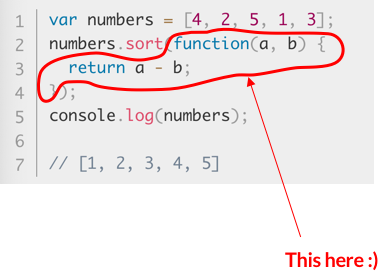
\includegraphics[width=0.8\linewidth]{images/part_1_notes_1.png}
    \end{center}

    \item In Java, to accomplish the above, used comparator interface with compare method
    \item Uses a lot of lines, an
    \begin{center}
    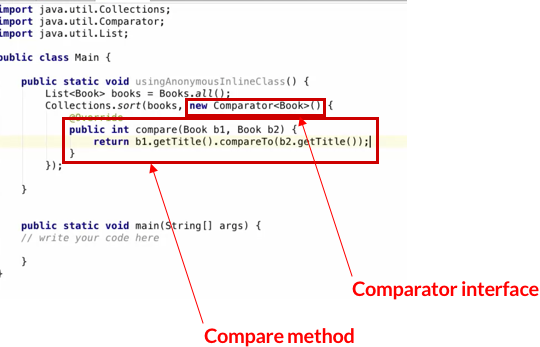
\includegraphics[width=0.8\linewidth]{images/part_1_notes_2.png}
    \end{center}
    \item Solution $\to$ Lambda
\end{itemize}


\end{document}